%Empieza configuracion de capitulo
\setstretch{1.0}
\titleformat{\chapter}[block]{\Large\bfseries}{CAP'ITULO \Huge\thechapter\vspace{25 pt}}{0 pt}{\\\fontsize{26}{36}\selectfont}
\titlespacing{\chapter}{0 pt}{30 pt}{50 pt}[0 pt]
\titleformat{\section}{\Large\bfseries}{\thesection}{0 pt}{\hspace{30 pt}}
\titleformat{\subsection}{\large\bfseries}{\thesubsection}{0 pt}{\hspace{30 pt}}
\pagestyle{fancy}
\fancyhead[LO,LE]{\footnotesize\textit{\leftmark}}
\fancyhead[RO,RE]{\thepage}
\fancyfoot[CO,CE]{}
%Termina configuracion de capitulo

\chapter{Marco Te'orico}
\setstretch{1.5} %Regresa el interlineado a 1.5

\normalsize

\section{Nociones B'asicas de Calidad de Software}
\noindent
En esta secci'on se dar'an las nociones b'asicas que se deben de conocer en el tema de la Calidad de Software antes de poder hablar de temas m'as espec'ificos.

\subsection{Definici'on de Calidad de Software}
\noindent
El concepto de Calidad de Software ha sido definido de varias formas por distintos autores. A continuaci'on se proveen algunas de las definiciones m'as destacables:

\begin{itemize}
	\item ``Calidad significa cumplir con los requerimientos'' - \cite{Crosby1979};
	\item ``Calidad consiste en las caracter'isticas de los productos que cubren las necesidades de los clientes produciendo satisfacci'on gracias al producto'' - \cite{Juran1988};
	\item ``Calidad consiste en la libertad de deficiencias'' - \cite{Juran1988};
	\item ``Calidad de Software es: El grado en que un sistema, componente o proceso cumple con los requerimientos especificados'' - IEEE 1991;
	\item ``Calidad de Software es: El grado en que un sistema, componente o proceso cumple con las necesidades o expectativas del usuario'' - IEEE 1991;
	\item ``Como la belleza, todos tienen su idea de que es la calidad'' - \cite{Davies2000}.
\end{itemize}

Tomando en cuenta estas definiciones, hay autores que se inclinan por definir Calidad de Software en relaci'on al cumplimiento de requerimientos, y otros que prefieren relacionar la calidad con la satisfacci'on final del cliente. Finalmente las empresas deben de buscar un balance apropiado entre ambos enfoques para lograr el 'exito en su labor.

\section{Enfoques de la Calidad de Software}
\noindent
Existen tres principales enfoques bajo los cuales la industria busca mejorar la calidad en el desarrollo de software. Estos son: Adherencia a procesos, elaboraci'on de pruebas y revisiones de producto.

\subsection{Adherencia a Procesos}
\noindent
Un enfoque que se tiene para dar calidad a los sistemas de software se hace mediante la definici'on y adherencia a procesos. La idea de este enfoque es que las organizaciones tengan procesos bien definidos, y los sigan religiosamente. Esto con el objetivo de siempre poder obtener resultados similares en sus diferentes procesos.

Dos grandes ejemplos de este enfoque son el ISO9000 el modelo de capacidad y madurez integrado (Por sus siglas en Ingl'es, CMMI).

ISO9000 es una familia de est'andares relacionados a la administraci'on de la calidad de los sistemas, y est'an dise'nados para ayudar a las organizaciones a asegurarse que cumplen con las necesidades de los clientes y las dem'as partes interesadas. Los est'andares que componen al ISO900 son \cite{Herzwurm1996}:

\begin{itemize}
	\item \emph{ISO9000}. Es la introducci'on al ISO 9000, se refiere a la selecci'on y uso de los ISO9001-9004;
	\item \emph{ISO9001}. Modelo para asegurar la calidad en el dise'no, desarrollo, producci'on e instalaci'on en las organizaciones;
	\item \emph{ISO9002}. Modelo para asegurar la calidad en la producci'on, instalaci'on y servicio. Est'a basado en el ISO9001 pero tambi'en incluye la parte de creaci'on de nuevos productos;
	\item \emph{ISO9003}. Modelo para asegurar la calidad en las inspecciones finales y el proceso de pruebas;
	\item \emph{ISO9004}. Modelo para asegurar la calidad a trav'es de situaciones preventivas.
\end{itemize}

CMMI es un modelo de referencia que gu'ia iniciativas de mejora de procesos que tiene como meta ayudar a las empresas a mejorar su desempe'no. Este modelo contiene los elementos esenciales de los procesos efectivos, y describe un proceso evolutivo  de mejora tanto para mejorar procesos inmaduros como para mejorar procesos maduros. Cuenta con 5 niveles de madurez que son los siguientes\cite{Yoo2005}:

\begin{itemize}
	\item \emph{Nivel 1 (Inicial)}. Procesos impredecibles, poco controlados y que reaccionan a las situaciones;
  \item \emph{Nivel 2 (Administrado)}. Proceso caracterizado por estar orientado a nivel proyecto, normalmente es reactivo a las situaciones;
	\item \emph{Nivel 3 (Definido)}. La organizaci'on tiene procesos definidos y es proactiva. Los proyectos se rigen mediante los procesos de la organizaci'on;
	\item \emph{Nivel 4 (Administrado Cuantitativamente)}. Los procesos de la organizaci'on son controlados y medidos cuantitativamente;
	\item \emph{Nivel 5 (Optimizaci'on)}. Se enfoca en la mejora continua de procesos.
\end{itemize}

\subsection{Pruebas de Software}
\label{sec:pruebasdesoftware}
\noindent
Un segundo enfoque es aquel que est'a basado en la realizaci'on de pruebas para asegurar la calidad del sistema. Las pruebas de software incluyen un proceso de verificaci'on y validaci'on de un sistema de software. Estas actividades se realizan con el objetivo de encontrar defectos en un sistema de software. Un defecto es una diferencia entre el resultado esperado y el resultado obtenido. 

Las pruebas de software son realizadas para encontrar los defectos en el sistema de software antes de que estos lleguen al usuario final. Existen distintos tipos de pruebas de software, los m'as comunes son \cite{JohnE.Bentley}:

\begin{itemize}
	\item \emph{Pruebas Unitarias}. Son pruebas ejecutadas a una unidad de sistema. Dependiendo del tipo de proyecto, una unidad puede ser considerada, un m'etodo dentro de alguna clase, un archivo de c'odigo fuente completo entre otras. En estas pruebas solo se asegura la funcionalidad asociada a la unidad.
	\item \emph{Pruebas de Sistema}. Es ejecutar todas las pruebas unitarias en un escenario real. Se refieren a utilizar el sistema bajo condiciones normales donde las unidades interact'uen entre s'i.
	\item \emph{Pruebas de Estr'es}. Es ejecutar pruebas de sistema pero bajo condiciones de estr'es, con una carga de trabajo muy alta y fuera de lo normal.
	\item \emph{Pruebas de Aceptaci'on de Usuari}o. Tambi'en conocidas como pruebas Beta, tratan de darle una versi'on funcional, aunque no propiamente final,  del sistema al usuario final, para que estos se aseguren de que el sistema hace lo que ellos necesitan y lo haga de forma correcta.
	\item \emph{Pruebas de Regresi'on}. Estas pruebas se ejecutan cuando se realiza la correcci'on de alg'un defecto. Todos los componentes o unidades que son afectados por este cambio tienen que ser probados de nuevo para asegurarse de que la correcci'on del defecto original no introdujo nuevos defectos.
\end{itemize}

Considerar los tipos de prueba c'omo la 'unica alternativa para remover defectos es inadecuado, costoso, poco efectivo y conlleva a perder el control del proyecto en la fase de pruebas. El enfoque de este Trabajo de Tesis es justamente evitar hacer pruebas extensivas. Como se mencion'o en la secci'on \ref{sec:planteamientodelproblema} del presente Trabajo de Tesis, gran parte de la problem'atica actual se debe a que los productos del proceso de desarrollo de software tienen una alta densidad de defectos por lo que llegan con una calidad muy baja a la etapa de pruebas, que a las organizaciones de desarrollo normalmente les toma la mitad del tiempo total del proyecto terminar esta etapa \cite{Humphrey2002}. El Trabajo de Tesis se enfoca en la revisi'on y prevenci'on de defectos durante el ciclo de vida, con el 'ultimo objetivo de que los productos del proceso de desarrollo de software lleguen libres de defectos a la etapa de pruebas.

\subsection{Revisiones de Productos de Trabajo}
\noindent
Las revisiones de los productos de trabajo son evaluaciones y revisiones de los productos creados durante el ciclo de vida de desarrollo de software ya sea de forma personal, o por parte de uno o m'as compa'neros del equipo de desarrollo calificados para hacerlo. Este es el enfoque del Trabajo de Tesis.

La idea principal detr'as de las revisiones es detectar los defectos lo antes posible en el proceso de desarrollo de software. Esto evita que los errores permanezcan durante el proceso de desarrollo, donde se multiplican y se va haciendo m'as dif'icil encontrarlos y corregirlos mientras avanza el proyecto\cite{McConnell2004}.

Los tipos de revisiones de productos m'as comunes son: Revisiones personales y entre colegas; caminatas e inspecciones. En la subsecci'on \ref{sec:tecnicasdedetecciondedefectos} del presente Trabajo de Tesis se esbozar'an distintas estrategias para promover la cultura de la revisi'on y la prevenci'on.

\section{Importancia de la Calidad en el Desarrollo de Software}
\noindent
El software es una tecnolog'ia sorprendente. Es un producto totalmente intelectual, aparte puede ser distribuido mundialmente en segundos, no se deteriora con el tiempo y es la forma m'as econ'omica y sencilla de implementar casi cualquier funci'on compleja.

En todos los campos de la ingenier'ia y la ciencia, m'as de la mitad del tiempo de cualquier profesional lo utiliza desarrollando, mejorando, manteniendo o usando un sistema de software. Es sin duda uno de los negocios m'as grandes e importantes de la actualidad\cite{Humphrey2002}.

Tomando en cuenta lo anterior, muchos ejecutivos de varias organizaciones vieron las oportunidades de negocio en el software, sin embargo implementar un departamento de software efectivo no es una tarea trivial, y la calidad en los productos que se desarrollen es clave para el 'exito.

\subsection{El software en las organizaciones}
\noindent
Para administrar una organizaci'on o un departamento dentro de una organizaci'on dedicado al software se necesita tener en cuenta los siguientes principios de administraci'on\cite{Humphrey2002}:

\begin{enumerate}
	\item Reconocer la importancia del software en el negocio;
	\item La calidad en los productos de software debe de ser la principal prioridad. La calidad es una elecci'on con consecuencias econ'omicas, si no se paga por la calidad al principio del desarrollo, se pagar'a una cantidad mucho m'as alta despu'es. Para realmente lograr que los proyectos cumplan con los calendarios y los costos, el trabajo tiene que realizarse de forma correcta desde el principio;
	\item El software de calidad se desarrolla por personas disciplinadas y motivadas. Si los profesionales del software no est'an convencidos y entrenados en m'etodos de calidad, no van a seguir las pr'acticas requeridas y no producir'an software de calidad.
\end{enumerate}

\subsection{?`Por qu'e los proyectos de software fallan?}
\noindent
La raz'on principal por la que los proyectos fallan es administraci'on inadecuada. Una buena administraci'on requiere dos cosas: Estar enfocados en la calidad, e ingenieros motivados que realicen un trabajo disciplinado. Las causas m'as comunes por las cuales los proyectos fallan son\cite{Humphrey2002}:

\begin{itemize}
	\item \emph{Calendarios poco realistas}. Cuando un proyecto de software inicia con calendarios poco realistas, el proyecto ser'a entregado despu'es de lo que se hubiera hecho con un calendario realista. Esto es porque los ingenieros comienzan a hacer trabajo r'apido y de poca calidad para alcanzar el calendario. El resultado de esto son productos de baja calidad, los cuales est'an llenos de defectos, lo que se traduce a una extensa etapa de pruebas;
	\item \emph{Equipo inadecuado}. La 'unica forma de terminar un proyecto de software de manera r'apida y efectiva es asignar el n'umero adecuado de personas y protegerlas de interrupciones y distracciones;
	\item \emph{Cambio de requerimientos}. Es normal que los requerimientos cambien en las fases iniciales del proyecto, sin embargo llega un punto que esta situaci'on es muy perjudicial. Se tiene que identificar este punto para evitar p'erdidas de dinero y cambios que afecten en sobremanera el trabajo que se est'a haciendo;
	\item \emph{Baja calidad en el trabajo realizado}. Si el trabajo que se realiza es de baja calidad, va a ocasionar que la fase de pruebas sea muy larga y se gaste mucho tiempo arreglando defectos durante el proceso de desarrollo;
	\item \emph{Creer en la magia}. No existe la bala de plata. Muchas veces se cree que con una nueva tecnolog'ia o forma de desarrollo resolver'a todos los problemas, y lo que ocurre generalmente es que pueden llevar a serios problemas.
\end{itemize}

El costo de una baja calidad de software es dif'icil de ver hasta el final del proyecto. Com'unmente, la baja calidad le dar'a problemas a'un a los usuarios finales ya que el proyecto se haya terminado. Los errores m'as comunes son: l'ideres de proyecto que toman compromisos irresponsables y no insisten en que el trabajo se haga de forma correcta. Todos los problemas mencionados anteriormente se pudieron evitar si la administraci'on hubiera insistido en planear correctamente el trabajo y realizarlo de forma disciplinada.

\subsection{La Calidad es Negocio}
\noindent
Hay tres razones fundamentales para insistir en que la Calidad de Software tiene que ser medida y administrada\cite{Humphrey2002}:

\begin{enumerate}
	\item La baja calidad en el software puede causar da'nos severos a la propiedad, y en algunos casos puede matar personas;
	\item El trabajo de calidad ahorra tiempo y dinero;
	\item Si la gerencia y el l'ider de proyecto no insisten en la administraci'on de la calidad de software, nadie m'as lo har'a.
\end{enumerate}

Varios estudios han demostrado que incluso los ingenieros experimentados inyectan un defecto cada diez l'ineas de c'odigo\cite{Humphrey2002}. Esto no significa que los programadores sean incompetentes, simplemente son humanos.

El costo de encontrar y corregir los defectos se incrementa en cada fase del proceso de desarrollo de software. Entre m'as permanezca un defecto en el sistema, ser'a m'as dif'icil removerlo, a dem'as de que se multiplica.

Existen varias t'ecnicas para remover defectos antes de llegar a la fase de pruebas. Estas t'ecnicas fueron  ser'an descritas a mayor profundidad en la secci'on \ref{sec:tecnicasdedetecciondedefectos} . Una de estas t'ecnicas por ejemplo, es la revisi'on de c'odigo, en las que se lee y revisa el c'odigo producido en busca de defectos. Estas actividades suelen tomar una peque'na cantidad de tiempo, y cada defecto encontrado ahorra una gran cantidad de tiempo en la fase de pruebas.

A diferencia de las revisiones de c'odigo, la fase de pruebas es una actividad de calidad mucho m'as larga. La raz'on de esto es que en las pruebas de software solo se revela los s'intomas del defecto, mientras que en las revisiones se encuentra directamente el defecto.

La mejor manera de remover defectos de software es realizando revisiones de c'odigo, ya que estas son m'as baratas y m'as efectivas que las pruebas de software. Adicionalmente, el ingeniero que desarroll'o el programa es el m'as indicado para encontrar y corregir sus propios defectos.

Aun conociendo la efectividad de las revisiones de c'odigo, muchas organizaciones no las utilizan. La raz'on es que para realizar revisiones de c'odigo efectivas se requieren m'etodos disciplinados.

Si los proyectos tienen la mayor parte de su tiempo dedicado a la fase de pruebas de software, va a ser casi imposible planearlo y darle seguimiento. Si se desea que los planes tengan compromisos precisos y realizables, se debe de insistir en realizar un trabajo de calidad incluyendo actividades de detecci'on de defectos.

\subsection{Introduciendo la Calidad a las Organizaciones}
Una organizaci'on exitosa siempre busca mejorar sus procesos por medio de reducir el tiempo que toman, aumentar su calidad y reducir sus costos. Un principio b'asico de la administraci'on que nos permite llegar a este objetivo es: Lo que se mide puede ser administrado y lo que es administrado puede ser realizado. Al contrario, lo que no es medido com'unmente se ignora. 

Para que una organizaci'on pueda construir software utilizando procesos de calidad que resulten en sistemas de alta calidad, debe de utilizar la administraci'on racional. El principio de administraci'on racional es confiar en que los miembros de un equipo de desarrollo de software son profesionales preocupados por el 'exito del proyecto. En la administraci'on racional se necesita crear planes, seguir estos planes, y corregir los problemas antes de que se salgan de control, tambi'en hace un 'enfasis especial en el calendario, la calidad y los costos. Los cuatro elementos principales de la administraci'on racional son\cite{Humphrey2002}:

\begin{enumerate}
	\item Establecer metas agresivas a largo plazo, pero descomponerlas en metas real'isticas y medibles a corto plazo;
	\item Insistir en la creaci'on de planes e insistir que estos planes sean creados por las personas que har'an el trabajo. Los planes tienen que ser detallados y completos, y tienen que ser revisados a conciencia en busca de omisiones y otros errores por los l'ideres de proyecto y la gerencia;
	\item Los planes de trabajo deben de ser utilizados al momento de realizar el trabajo. Esto permite realizar balanceo de cargas y conocer el estado actual del proyecto. Todos los productos deben de tener alta calidad, si no es as'i eventualmente tendr'an que ser corregidos y tendr'an un costo extra.
	\item Se tienen que utilizar datos e informaci'on. Si se utiliza de forma objetiva los datos y la informaci'on del desempe'no del equipo, se demuestra la confianza que se tiene en el equipo y la disposici'on que existe para escuchar sus problemas, planes e ideas;
	\item La reducci'on de costos se logra por medio de maximizar el tiempo de trabajo de los ingenieros, y esto se hace planeando el tiempo que tomar'an las actividades y midiendo el tiempo que realmente tomaron.
	\item Dar seguimiento al trabajo realizado y  utilizar la informaci'on actual para anticipar y resolver problemas futuros. Los calendarios y planes se salen de control d'ia a d'ia.
\end{enumerate}

En resumen, para que una organizaci'on pueda mejorar su calidad las diferentes partes deben de cumplir con lo propuesto anteriormente. Los ingenieros deben de utilizar las pr'acticas de calidad, as'i como planear y dar seguimiento al trabajo realizado y finalmente medir y administrar la calidad del producto. Los l'ideres o administradores de proyecto deben iniciar y mantener este nuevo comportamiento, as'i como monitorear los planes y balancear efectivamente la carga de trabajo. La gerencia o l'ideres de la organizaci'on deben de proveer un ambiente disciplinado y atractivo de trabajo, establecer las metas a largo plazo y dar seguimiento al trabajo realizado. Cuando el trabajo es planeado, medido y monitoreado, se puede analizar el desempe'no del proyecto y del negocio.

El BM proveer'a a las organizaciones con la infraestructura b'asica para la implementaci'on de una administraci'on racional. Permitir'a establecer planes, dar de alta tareas con sus tiempos planificados, darles seguimiento y registrar sus tiempos reales. M'as detalles de esto se dar'an en la secci'on \ref{sec:administracionyseguimientodeactividades}.

\subsection{Beneficios del Trabajo de Calidad}
\noindent
Cuando se utilizan correctamente m'etodos disciplinados para planear, dar seguimiento y administrar, el trabajo ser'a de alta calidad y ser'a terminado dentro de calendario. M'as importante a'un, tendremos una noci'on bastante precisa de en qu'e parte del proceso de desarrollo se encuentra el proyecto, y una predicci'on fiable de cu'ando se va a terminar.

El tiempo que se requiere para escribir programas de alta calidad es el mismo que se necesita para escribir programas de baja calidad. Los productos de calidad reducen el tiempo desarrollo. Entre menos defectos existan, el costo ser'a menor y los estimados ser'an m'as efectivos. Tambi'en el tiempo que se requiera para terminar la etapa de pruebas ser'a mucho menor.

\section{El Proceso Personal del Software}
\noindent
El Proceso Personal del Software (por sus siglas en Ingl'es PSP) es una metodolog'ia de mejora continua en el desarrollo de software propuesta por Watts Humphrey en su libro ``PSP A Self-Improvement Process for Software Engineers''\cite{Humphrey}. El PSP ayuda a controlar, administrar y mejorar los procesos para desarrollar software. Provee una infraestructura de gu'ias, plantillas y procedimientos para: desarrollar software, dar seguimiento a los defectos y admistrar la calidad. Esto hace que los productos de trabajo sean m'as predecibles y eficientes, que se elaboren mejores planes, dar un seguimiento adecuado al desempe'no y medir la calidad de los productos elaborados.

El BM toma varios conceptos de esta metodolog'ia para alcanzar los objetivos que propone. En esta secci'on ser'an descritos los conceptos de los que hace uso el BM.

\subsection{?`Qu'e es la calidad de software?}
\noindent

Los m'etodos tradicionales para asegurar la calidad del software en desarrollo son: Inspecci'on de requerimientos, inspecci'on de dise'no, compilaci'on, inspecci'on de c'odigo y pruebas. La tabla \ref{DefectosNivelCMM} muestra los niveles de defectos promedio por las organizaciones seg'un su nivel de CMM\cite{Humphrey}.

\begin{table}[htbp]
	\centering
		\begin{tabular}{| c | c |}
			\hline
			\textbf{Nivel de CMM} & \textbf{Defectos/Mil de L'ineas de C'odigo} \\ \hline
			1 & 7.5 \\ \hline
			2 & 6.24 \\ \hline
			3 & 4.73 \\ \hline
			4 & 2.228 \\ \hline
			5 & 1 \\ 
			\hline
		\end{tabular}
	\caption{N'umero de Defectos por Nivel de CMM}
	\label{DefectosNivelCMM}
\end{table}

Para mejorar la calidad de productos de software, aparte de utilizar los m'etodos tradicionales de calidad, se debe de medir y dar seguimiento al trabajo personal. S'i el objetivo es tener un sistema de software de alta calidad, cada parte del sistema debe de ser de alta calidad. La estrategia de PSP es administrar los defectos contenidos en todas las partes del sistema. Con partes de alta calidad, el proceso de desarrollo de software se puede escalar sin perder productividad.

La definici'on de calidad deber'ia de basarse en las necesidades de los usuarios\cite{Humphrey}. Los usuarios deben de contar con un producto funcional. Si el producto tiene muchos defectos este no se desempe'nar'a con una consistencia razonable. Sin embargo esto no significa que los defectos son siempre la principal prioridad. Despu'es de los defectos se tienen caracter'isticas de calidad como: Desempe'no, seguridad, usabilidad, compatibilidad, funcionalidad, confiabilidad entre otras. Normalmente se gasta un tiempo excesivo en la correcci'on de defectos, dejando muy poco tiempo dedicado a las otras caracter'isticas mencionadas anteriormente.

Aunque los defectos son solo una parte de la calidad del producto de software, son el principal objetivo del PSP, ya que la administraci'on efectiva de estos es esencial para la administraci'on de costo, calendario y los dem'as aspectos de la calidad de producto.

\subsection{La Econom'ia de la Calidad de Software}
\noindent
La calidad de software es un problema de econ'omico. Cada prueba realizada cuesta dinero y toma tiempo. Entre m'as tiempo el defecto permanezca en el producto, el impacto es m'as alto. Por ejemplo encontrar un problema de requerimientos cuando el cliente ya est'a utilizando el producto puede ser demasiado costoso; en cambio, encontrar el defecto durante una revisi'on de c'odigo ser'a mucho menos costoso. El objetivo, entonces, es remover los defectos lo antes posible en el proceso de desarrollo. Esto se logra haciendo revisiones e inspecciones de cada producto de trabajo lo m'as pronto posible, antes de que se haya terminado de construir el producto de software.

El proceso de pruebas puede ser muy efectivo para identificar problemas de desempe'no, usabilidad y problemas operacionales, pero no es tan efectivo removiendo grandes cantidades de defectos. Los datos de estudios realizados demuestran que mientras m'as tarde en el proceso de desarrollo sea encontrado un defecto, es m'as dif'icil encontrarlo y removerlo\cite{Humphrey}. La tabla \ref{CostoEncontrarCorregir} nos muestra cuanto cuesta encontrar y corregir defectos en Inspecciones, Pruebas y Mantenimiento seg'un distintos estudios:

\begin{table}[htbp]
	\centering
		\begin{tabular}{| c | c | c | c |}
			\hline
			\textbf{Referencia} & \textbf{Inspecci'on} & \textbf{Pruebas} & \textbf{Uso} \\ \hline
			IBM (Remus and Ziles 1979) \cite{Remus1979} & 1 & 4.1 veces la inspecci'on &  \\ \hline
			JPL (Bush 1990)\cite{Bush1990} & \$90 - \$120 & \$10,000 &  \\ \hline
			Ackerman et al. 1989\cite{Ackerman1989} & 1 hora & 2-20 horas &  \\ \hline
			Ragland 1992\cite{Ragland1992} &  & 20 horas &  \\ \hline
			Russell 1991\cite{Rusell1991} & 1 hora & 2-4 horas &  \\ \hline
			Shooman and Bolsky 1975\cite{Shooman1975} & 0.6 horas & 3.05 horas &  \\ \hline
			Weller 1993\cite{Weller1993} & 0.7 horas & 6 horas &  \\ 
			\hline
		\end{tabular}
	\caption{Costo de Encontrar y Corregir Defectos}
	\label{CostoEncontrarCorregir}
\end{table}

\subsection{Tipos de Defectos}
\noindent
Los tipos de defectos m'as comunes son: Errores en requerimientos, errores de dise'no, errores de codificaci'on, errores de documentaci'on, correcciones defectuosas. La tabla \ref{TiposDefectosKLOC} presenta el n'umero de defectos cada mil l'ineas de c'odigo seg'un el tipo de defecto\cite{Humphrey}.

\begin{table}[htbp]
	\centering
		\begin{tabular}{| c | c |}
			\hline
			\textbf{Tipos de Defecto} & \textbf{Defectos/Mil de L'ineas de C'odigo} \\ \hline
			Requerimientos & 2.3 \\ \hline
			Dise'no & 1.9 \\ \hline
			Codificaci'on & 0.9 \\ \hline
			Documentaci�n & 1.2 \\ \hline
			Correcciones Defectuosas & 1.2 \\ \hline
			Total & 7.5 \\
			\hline
		\end{tabular}
	\caption{Tipos de Defectos por Mil L'ineas de C'odigo}
	\label{TiposDefectosKLOC}
\end{table}

\subsection{M'etricas de Calidad}
\noindent
Para mejorar la calidad, se debe de medir la calidad\cite{Humphrey}. El PSP propone el uso de las siguientes m'etricas para medir la calidad de las organizaciones de software: La efectividad de la t'ecnica de detecci'on de defectos (Yield de Calidad), el Costo de la Calidad (Por sus siglas en Ingl'es, COQ), la Tasa de Revisiones, la Calidad de Radio de Fases y el 'Indice de Calidad de Proceso.

El Yield mide la eficiencia de cada fase en la detecci'on de defectos. El Yield de una fase es el porcentaje de defectos de producto totales que son removidos en esa fase. El Yield de proceso es el porcentaje de defectos que son removidos antes de la primera compilaci'on o pruebas de unidad. El Yield de proceso aumenta claramente cuando se comienzan a utilizar revisiones de dise'no y de c'odigo.

El COQ tiene tres componentes principales\cite{Humphrey}:

\begin{enumerate}
	\item \emph{Costo de las Fallas (CF)}. El costo total de las fases de compilaci'on y de pruebas;
	\item \emph{Costos de Evaluaci'on (CE)}. El tiempo utilizado en revisiones de c'odigo y de dise'no;
	\item \emph{Costos de Prevenci'on}. El costo de identificar causas de defectos y acciones para prevenirlos en el futuro.
\end{enumerate}

En la tabla \ref{MetricasCOQ} se muestran las m'etricas que se pueden obtener a partir del an'alisis del COQ\cite{Humphrey}.

\begin{table}[htbp]
	\centering
		\begin{tabular}{|l|l|l|} \hline
		\multicolumn{3}{|c|}{\textbf{F'ormulas COQ}} \\ \hline
		\multirow{4}{*}{\begin{math}CF = 100(\frac{TC + TP}{TTD})\end{math}} 
		& CF & Costo de Fallas \\
		& TC & Tiempo de Compilaci'on \\
		& TP & Tiempo de Pruebas \\
		& TTD & Tiempo Total de Desarrollo \\ \hline
		\multirow{4}{*}{\begin{math}CE = 100(\frac{TRD + TRC}{TTD})\end{math}} 
		& CE & Costo de Evaluaci'on \\
		& TRD & Tiempo de Revisi'on de Dise'no \\
		& TRC & Tiempo de Revisi'on de C'odigo \\
		& TTD & Tiempo Total de Desarrollo \\ \hline
		\multirow{2}{*}{\begin{math}TCOQ = CF + CE\end{math}} 
		& CE & Costo de Evaluaci'on \\
		& CF & Costo de Fallas \\ \hline
		\multirow{2}{*}{\begin{math}CE\% = 100(\frac{CE}{TCOQ})\end{math}} 
		& CE & Costo de Evaluaci'on como \% del TTD\\
		& TCOQ & Costo Total de la Calidad \\ \hline
		\multirow{3}{*}{\begin{math}RF = \frac{CE}{CF}\end{math}} 
		& RF & Raz'on de Falla \\
		& CE & Costo de Evaluaci'on \\
		& CF & Costo de Fallas \\ \hline		
		\end{tabular}
	\caption{M'etricas del COQ}
	\label{MetricasCOQ}
\end{table}

El Yield y el COQ son 'utiles, pero miden el trabajo que hiciste, no lo que est'as haciendo. La Tasa de Revisi'on y el Radio de Calidad por Fase proveen una manera de dar seguimiento y control a los tiempos de revisi'on. 

La tasa de revisi'on se utiliza principalmente para revisiones de c'odigo e inspecciones, y mide el n'umero de L'ineas de C'odigo (LOC por sus siglas en Ingl'es) o p'aginas revisadas por hora.

El Radio de Calidad por Fase, Es el radio de tiempo utilizado en dos fases de proceso. El radio para la revisi'on es el tiempo utilizado para realizar revisiones dividido entre el tiempo de desarrollo.

El 'Indice de Calidad de Proceso (PQI por sus siglas en Ingl'es), es una m'etrica compuesta por cinco sub-m'etricas, la cual nos permite analizar el desempe'no general de los procesos de una organizaci'on de software. El PQI se obtiene de multiplicar las cinco sub-m'etricas que se presentan en la tabla \ref{SubMetricasPQI}. El valor ideal es que el resultado sea 1.0; sin embargo, estudios realizados por Humphrey\cite{Humphrey} indican que un valor mayor a 0.4 provee un valor adecuado de calidad.

\begin{table}[htbp]
	\centering
		\begin{tabular}{|l|l|l|} \hline
		\multicolumn{3}{|c|}{\textbf{F'ormulas PQI}} \\ \hline
		\multirow{3}{*}{\begin{math}DP = \frac{TD}{TP}\end{math}} 
		& DP & PQI de Dise'no y Programaci'on \\
		& TD & Tiempo de Dise'no \\
		& TP & Tiempo Programaci'on \\ \hline
		\multirow{3}{*}{\begin{math}RD = 2(\frac{TRD}{TD})\end{math}} 
		& RD & PQI de Revisi'on de Dise'no \\
		& TRD & Tiempo de Revisi'on de Dise'no \\
		& TD & Tiempo de Dise'no \\ \hline
		\multirow{3}{*}{\begin{math}RP = 2(\frac{TRP}{TP})\end{math}} 
		& RP & PQI de Revisi'on de Programaci'on \\
		& TRP& Tiempo de Revisi'on de Programaci'on \\
		& TP & Tiempo de Programaci'on \\ \hline
		\multirow{3}{*}{\begin{math}DC = 20(10 + \frac{DC}{KLOC})\end{math}} 
		& DC & PQI para Defectos de Compilaci'on por KLOC\\
		& DC & Defectos de Compilaci'on \\
		& KLOC & Mil L'ineas de C'odigo \\ \hline
		\multirow{3}{*}{\begin{math}DT = \frac{10}{5 + \frac{DT}{KLOC}}\end{math}} 
		& DT & PQI para Defectos de Pruebas por KLOC \\
		& DT & Defectos de Pruebas \\
		& KLOC & Mil L'ineas de C'odigo \\ \hline	
		\multirow{1}{*}{\begin{math}TPQI = DP \cdot RD \cdot RP \cdot DC \cdot DT\end{math}} 
		& TPQI & PQI Total \\ \hline		
		\end{tabular}
	\caption{M'etricas del PQI}
	\label{SubMetricasPQI}
\end{table}

\subsection{Pr'acticas para la Mejora de Calidad del PSP}
\noindent

Existen seis principios que recomienda el PSP para la Mejora de la Calidad Personal\cite{Humphrey}:

\begin{enumerate}
	\item Para tener calendarios predecibles, se tiene que planear y dar seguimiento al trabajo personal;
	\item Para hacer planes precisos y que se les pueda dar seguimiento, estos planes tienen que ser detallados;
	\item Para hacer planes detallados, se deben basar en datos hist'oricos;
	\item Para hacer un trabajo de alta calidad, se debe usar un proceso personal definido y medible;
	\item Ya que el trabajo de mala calidad no es predecible, la calidad es un pre requisito para la predictibilidad.
\end{enumerate}

Estos principios se promueven en el BM porque provee la infraestructura para dar seguimiento al trabajo personal, almacena datos hist'oricos y permite el establecimiento de ciclos de vida.

\subsection{Prevenci'on de Defectos}
\noindent

Para prevenir la inyecci'on de defectos se debe de revisar los datos de los defectos que m'as se encuentran durante el desarrollo y las pruebas. Esto nos ayuda a conocer cuales son los defectos m'as comunes y establecer estrategias como enfocarse en los errores que:

\begin{itemize}
	\item Se encuentran en el programa final o en el periodo de pruebas;
	\item Aquellos que ocurren m'as frecuentemente;
	\item Aquellos que son m'as dif'iciles o costosos de corregir;
	\item Aquellos en los que se pueden realizar acciones preventivas sencillas;
	\item Aquellos que m'as nos molestan.
\end{itemize}

El BM est'a basado en esta filosof'ia. Fomenta las ideas de realizar revisiones personales a los programas. La revisi'on de defectos se hace con el fin de detectar los defectos, sin embargo no es suficiente, el BM tambi'en recomienda su registro, seguimiento y administraci'on. Al registrar los defectos podemos generar estad'isticas y reportes que permitan conocer los tipos de defectos mencionados anteriormente.

\subsection{T'ecnicas de Detecci'on de Defectos}
\label{sec:tecnicasdedetecciondedefectos}
\noindent
Las t'ecnicas de detecci'on de defectos pueden ser definidas como la evaluaci'on y la revisi'on de un producto de trabajo por parte de uno o m'as compa'neros de trabajo calificados para realizar la actividad\cite{Owens1997}.

Existen diferentes tipos de t'ecnicas de detecci'on de defectos, unas m'as formales y r'igidas que otras. Evidentemente la diferencia radica en la forma de conducir la revisi'on del producto de trabajo. Tambi'en existen diferentes clasificaciones acerca de las t'ecnicas. Una posible clasificaci'on consiste en separar las t'ecnicas que involucran a una sola persona y las t'ecnicas en las que participan dos o m'as miembros del equipo. Los tipos m'as utilizados son: La revisi'on personal y la revisi'on entre colegas.

La revisi'on personal consiste en examinar el producto de trabajo antes de entregarlo a cualquier otro miembro del equipo, ya sea para su lectura, compilaci'on, revisi'on, implementaci'on o prueba.

Existen varias t'ecnicas de detecci'on de defectos que se realizan entre colegas y/o miembros de un equipo de desarrollo\cite{Harjumma2005}. Estas t'ecnicas se puede clasificar de acuerdo a su formalidad, de acuerdo \cite{Harjumma2005} con existen 6 diferentes tipos de t'ecnicas:

\begin{itemize}
	\item Revisi'on ad hoc;
	\item Revisi'on general;
	\item Revisi'on de parejas;
	\item Revisi'on de equipo;
	\item La Caminata y la inspecci'on son explicadas m'as detalladamente a continuaci'on.
\end{itemize}

La caminata es un tipo de revisi'on en el que precisamente una persona (preparada especialmente para ello) pasa por cada una de las partes del producto, exponi'endolo a una audiencia. Mediante esta t'ecnica se pueden obviar muchos detalles, con lo cual se reduce el tiempo de revisi'on. Sin embargo, esto puede ser contraproducente si el objetivo es precisamente detectar defectos que residen en los detalles. Al mismo tiempo, el proceso de revisi'on est'a definido por el producto de trabajo siendo revisado, a diferencia de la inspecci'on, en el que el proceso se determina por los puntos a revisar\cite{Freedman1984}.

La Inspecci'on es probablemente la t'ecnica m'as formal de detecci'on de defectos de software\cite{Harjumma2005}. Consiste de los siguientes pasos\cite{Owens1997}:

\begin{enumerate}
	\item \emph{Planeaci'on}: Seleccionar d'onde, cu'ando y qui'enes participar'an;
	\item \emph{Resumen}: Revisi'on general para que los revisores se familiaricen con el producto de trabajo;
	\item \emph{Preparaci'on}: Cada revisor lee el producto de trabajo e identifica posibles defectos. Todo esto generalmente mediante listas de chequeo. La persona que realiza el papel de l'ider, se prepara para la junta de revisi'on;
	\item \emph{Junta}: El l'ider modera la junta y realiza la revisi'on del producto. Los revisores lo interrumpen para discutir los defectos encontrados. Lo m'as importante es que NO se permite discutir posibles soluciones para ning'un defecto;
	\item \emph{Re-trabajo}: El autor del producto realiza las correcciones pertinentes;
	\item \emph{Seguimiento}: El autor del producto notifica al l'ider de las correcciones y 'estas son revisadas. 
\end{enumerate}

Tanto la caminata como la inspecci'on aumentan su efectividad cuando se utilizan listas de chequeo. El BM permitir'a la creaci'on de plantillas que sirvan de gu'ia para la realizaci'on de estas t'ecnicas. La funcionalidad ser'a explicada m'as a detalle en la secci'on [REFERENCIA].

\subsection{?`Por qu'e Revisar los Programas?}
\noindent
Los programas se revisan porque es la manera m'as r'apida y m'as barata para encontrar y corregir problemas antes de dise'nar una funci'on equivocada o implementar un dise'no incorrecto. Un poco de tiempo invertido revisando un programa puede ahorrar mucho tiempo durante las fases de compilaci'on y pruebas. A'un m'as importante, cuando todos en el equipo de desarrollo hacen revisiones de dise'no y de c'odigo a conciencia, el tiempo de integraci'on y de pruebas de sistema es reducido en un factor de cinco a diez.

\subsection{Principios de la Revisi'on}
Los principios de las revisiones personales son los siguientes\cite{Humphrey}:

\begin{itemize}
	\item Revisar personalmente todo el trabajo propio antes de pasar a la siguiente fase de desarrollo;
	\item Intentar lo mejor posible corregir todos los defectos antes de dar el producto de trabajo a otra persona en el equipo de desarrollo;
	\item Utilizar una lista de chequeo personal y seguir un proceso estructurado de revisi'on;
	\item Seguir las buenas pr'acticas de la revisi'on: revisar en incrementos peque'nos, hacer las revisiones en papel y hacerlas cuando est'as descansado;
	\item Medir el tiempo de la revisi'on, el tama'no de los productos revisados y el n'umero y tipo de defectos encontrados y perdidos;
	\item Usar los datos de las mediciones para mejorar el proceso personal de revisi'on;
	\item Dise'nar e implementar los productos para que sean f'aciles de revisar;
	\item Revisar los datos para identificar las formas de prevenir defectos.
\end{itemize}

Esta es la herramienta principal que propone el BM para la detecci'on de defectos. El BM tiene una plantilla por default para realizar revisiones personales en lenguajes de programaci'on de prop'osito general. Esto se explica m'as a detalle en la secci'on [REFERENCIA].

\subsection{Lista de Chequeo de Revisi'on de C'odigo}
\noindent
Una lista de chequeo es una forma especializada que se usa para hacer las revisiones. La lista de chequeo tambi'en ayuda a disciplinar el trabajo y gu'iar en el proceso de revisi'on.

Para la revisi'on personal es necesario que cada persona desarrolle su propia lista de chequeo, para que cada persona se enfoque en los errores que m'as comete, o en los que quiere evitar seg'un la estrategia que se siga, y que se completen todos los elementos de la lista. Para hacer un mejor uso de la lista de chequeo se tiene que dividir la lista en secciones con caracter'isticas similares para concentrarte en los mismos tipos de errores en cada pasada al documento a revisar (ya sea c'odigo, dise'no o requerimientos). Para elaborar una lista de chequeo se puede tomar como base los tipos de defectos mostrados en la tabla \ref{DefectosPSP} \cite{Humphrey}.

\begin{table}[htbp]
	\centering
		\begin{tabular}{| l | l | l |}
			\hline
			\textbf{N'umero de Tipo} & \textbf{Nombre del Tipo} & \textbf{Descripci'on} \\ \hline
			10 & Documentaci'on & Comentarios y mensajes. \\ \hline
			20 & Sintaxis & Ortograf'ia, puntuaci'on y tipos. \\ \hline
			30 & Paquete & Administraci'on, librer'ias y versiones. \\ \hline
			40 & Asignaci'on & Declaraci'on, nombres duplicados y l'imites. \\ \hline
			50 & Interface & Procedimientos, referencias, I/O y formatos. \\ \hline
			60 & Chequeo & Mensajes de error y chequeos inadecuados. \\ \hline
			70 & Datos & Estructura y contenido. \\ \hline
			80 & Funci'on & L'ogica, apuntadores, ciclos, etc. \\ \hline
			90 & Sistema & Configuraci'on, tiempo y memoria. \\ \hline
			100 & Medio Ambiente & Dise'no, compilaci'on y pruebas.\\
			\hline
		\end{tabular}
	\caption{Clasificiaci'on de Defectos del PSP}
	\label{DefectosPSP}
\end{table}

La lista de chequeo es construida a partir de esta lista de defectos. Se deben proponer distintas actividades para enfocarse a remover los distintos tipos de defectos. La tabla \ref{ListaChequeoRevisionCodigoPSP} presenta un ejemplo de lista de chequeo para lenguajes de prop'osito general propuesta por Humphrey\cite{Humphrey}.

\begin{table}[htbp]
	\centering
		\begin{tabular}{|l|l|} \hline
		\multicolumn{2}{|c|}{\textbf{Lista de Chequeo para la Revisi'on de C'odigo}} \\ \hline
		\textbf{Nombre del Revisor} &  \\ \hline
		\textbf{Nombre del Programa} &  \\ \hline
		\textbf{Lenguaje} &  \\ \hline
		\textbf{Prop'osito} & Ser una gu'ia para la revisi'on de c'odigo \\ \hline
		\multirow{3}{*}{\textbf{General}} 
		& - Revisa el programa por cada categor�a. \\
		& - No intentar revisar dos categor�as a la vez. \\
		& -	Cada que se complete un paso palomear el cuadro. \\ \hline
		\textbf{Documentaci'on} & - Los m'etodos est'an documentados correctamente. \\ \hline	
		\multirow{3}{*}{\textbf{Sintaxis}} 
		& - Todas las l'ineas del programa terminan en ";" .\\
		& - Todas las llaves, corchetes y par'entesis tienen su pareja. \\
		& -	El c'odigo est'a correctamente indentado. \\ \hline
		\multirow{2}{*}{\textbf{Paquete}} 
		& - El programa se encuentra en la carpeta correcta.\\
		& -	Todas las librer�as requeridas est'an presentes. \\ \hline
		\multirow{4}{*}{\textbf{Asignaci'on}} 
		& - Las variables tienen el tipo de dato correcto.\\
		& - Las variables siguen las convenciones de nombrado.\\
		& - Todas las variables est'an inicializadas.\\
		& -	Las variables tienen el alcance adecuado.\\ \hline
		\multirow{3}{*}{\textbf{Interface}} 
		& - Los archivos le'idos o escritos existen.\\
		& -	Las llamadas a funciones son correctas. \\ \hline
		& - Las llamadas a funciones tienen los par'ametros adecuados. \\ \hline
		\multirow{2}{*}{\textbf{Chequeo}} 
		& - Los m'etodos utilizados manejan excepciones.\\
		& -	Los mensajes de error mandados son 'utiles. \\ \hline
		\multirow{2}{*}{\textbf{Datos}} 
		& - La base de datos utilizada existe.\\
		& -	Las consultas a la base de datos son correctas. \\ \hline
		\multirow{3}{*}{\textbf{Funci'on}} 
		& - La l'ogica de los m'etodos es correcta.\\
		& - Los apuntadores est'an definidos correctamente.\\
		& -	Los ciclos respetan el tama'no de los arreglos.\\ \hline
		\textbf{Sistema} & - El programa utiliza correctamente la memoria disponible.\\ \hline	
		\end{tabular}
	\caption{Lista de Chequeo para la Revisi'on de C'odigo de PSP}
	\label{ListaChequeoRevisionCodigoPSP}
\end{table}

La lista de chequeo aparte de ser personalizada, tiene que ser actualizada constantemente. La persona al seguir los procesos de calidad tiene una mejor'ia notable en la forma de hacer su trabajo, por lo tanto los errores que se comenten en el tiempo van cambiando y la lista tiene que ser actualizada. Tambi'en se tiene que tener en cuenta que las listas de chequeo cambian notablemente de un proyecto a otro, dependiendo del lenguaje de programaci'on que se utilice entre otros factores.

La intenci'on de la revisi'on de c'odigo es asegurar que todos los detalles son correctos. Una vez que se definen las pr'acticas, deben de ser incorporadas en los est'andares y ser checados en las revisiones.

La estrategia de la revisi'on es:

\begin{itemize}
	\item Para asegurar que el c'odigo cubre todo el dise'no, se revisa cada m'etodo para asegurar que todas las funciones requeridas est'an incluidas;
	\item Para checar las librer'ias a incluir, examinar cada m'etodo para asegurar que existan las inclusiones necesarias para cada funci'on de la librer'ia;
	\item Para checar problemas de inicializaci'on, realizar una caminata por la l'ogica de todos los m'etodos.
\end{itemize}

Esta estrategia debe de ser utilizada en las revisiones registradas en el BM.

\subsection{Evaluando las Revisiones Personales}
\noindent
Algunas medidas 'utiles para evaluar las revisiones son:

\begin{itemize}
	\item El tama'no del programa revisado;
	\item El tiempo de revisi'on en minutos;
	\item N'umero de defectos encontrados;
	\item N'umero de defectos en el programa que se encontraron despu'es, en otras palabras aquellos que no fueron encontrados en la revisi'on.
\end{itemize}

Las m'etricas formales que se proponen por PSP son: Yield de Revisi'on, Densidad de Defectos, Tasa de Defectos y Tasa de Revisi'on. 

Yield de revisi'on es el porcentaje de defectos en el producto que fueron encontrados en la revisi'on. Un Yield alto es bueno, uno malo es pobre. La meta del Yield debe de ser el 100\%. La meta de PSP es encontrar y corregir todos los errores antes de la primera compilaci'on o las pruebas; es decir, un yield de proceso ed 100\%. Para hacer un estimado de Yield para cualquier fase, debes de asumir el Yield de la fase anterior. Inicialmente es com'un un Yield de fase de 50\% y conforme se va madurando la t'ecnica es posible tener 70\% o m'as\cite{Humphrey}.

La Tasa de Defectos es el n'umero de defectos que se encontraron en el c'odigo por LOC.

La Tasa de Revisi'on es el n'umero de l'ineas que se revisan por hora. El ideal es entre 200 y 400 l'ineas por hora.

La efectividad de los m'etodos de revisi'on es el radio de defectos removidos por hora en la revisi'on.

\subsection{Efectividad de la Revisi'on}
\noindent
Las revisiones de c'odigos son inherentemente mejores que las pruebas\cite{Humphrey}. Depuraci'on es el proceso de encontrar c'odigo defectuoso que causa que el programa se comporte impropiamente. La cantidad de tiempo que se gasta realizando el debugging generalmente tiene poca relaci'on con la complejidad del defecto\cite{Humphrey}.

La meta de la revisi'on es remover el m'aximo n'umero de defectos, en otras palabras llegar a pruebas con cero defectos. En una revisi'on, personalmente se revisa el programa que una ha generado. Una inspecci'on es una revisi'on en equipo de un programa. Despu'es de las revisiones personales, la inspecci'on es la t'ecnica m'as valiosa que un equipo de desarrollo de software puede utilizar.

\subsection{Dise'no de Software}
\noindent
La principal herramienta a disposici'on de los ingenieros de software son las abstracciones. Se pueden crear abstracciones arbitrariamente y combinarlas en abstracciones m'as grandes. Si se cumplen con las capacidades de los sistemas que se soportan entonces tambi'en se pueden crear las estructuras l'ogicas que necesarias.

El principal problema reside en la escala o el tama'no de los sistemas de software. La forma de subdividir los sistemas tiene que ser coherente y realmente ayudar a resolver los problemas de complejidad. Ya que si en el caso de un sistema de 1,000,000 LOC, creas 500 tipos de 10 LOC, entonces tendr'ias que dise'nar un sistema de 100,000 LOC, lo que parece una ayuda, pero en realidad se forza a los dise'nadores a relacionar coherentemente los 500 tipos distintos. Para que la escalabilidad sea 'util, no solamente se debe de capturar los requerimientos f'isicos de la escalabilidad, si no capturar un nivel de funcionalidad significativa en las partes.

La forma m'as cl'asica es utilizar la regla de divide-y-vencer'as. En otras palabras, el sistema se tiene que dividir en partes m'as peque'nas, las cuales deben de ser vistas como subsistemas coherentes o componentes. Si esto se hace correctamente, se reduce la complejidad en un factor de diez o m'as.  Sin embargo hacer esto correctamente es una tarea dif'icil, a la que se llama dise'no. El dise'no de calidad tiene dos partes: la calidad del concepto de dise'no y la calidad de la representaci'on del dise'no.

Producir un dise'no claro, completo y libre de defectos es un paso necesario para construir productos de calidad. Crear dise'nos detallados hace m'as lento el proceso individual de desarrollo, sin embargo, si todo el equipo de desarrollo hace lo mismo, acelerar'a el trabajo en equipo ya que facilitar'a el trabajo de integraci'on y pruebas de sistema.

\subsection{El Proceso de Dise'no}
\noindent
El dise'no de software es una actividad creativa la cual no puede ser reducida a un proceso rutinario. Sin embargo, esta actividad, no tiene que carecer por completo de estructura. El dise'no generalmente inicia revisando el prop'osito del producto, obteniendo datos relevantes, produciendo una vista general del dise'no y llenando los detalles. Para dise'nos complejos, los buenos dise'nadores siguen un proceso din'amico. Ellos trabajan en un nivel conceptual por un periodo de tiempo y despu'es ahondan en cada parte.

Ocasionalmente, el dise'nador no va a ser capaz de especificar una funci'on hasta que se haya dise'nado, construido y probado. En estos casos se deben de construir prototipos para estas funciones. Antes de desarrollar un prototipo, se debe de especificar su prop'osito y las preguntas que va a responder.

\subsection{Niveles de Dise�o}
\noindent
Los diferentes niveles de dise'no son\cite{Humphrey}:

\begin{enumerate}
	\item \emph{El dise'no conceptual}. Es un concepto de planeaci'on que se utiliza para estimar el tama'no del producto.
	\item \emph{Dise'no de alto nivel (HLD)}. Este dise'no tiene como objetivo dividir el sistema que se est'a desarrollando en partes m'as peque'nas o componentes.
	\item \emph{Dise'no detallado (DLD)}. Este nivel de dise'no toma los componentes especificados por el HLD y define como construirlos.
\end{enumerate}

Los ciclos de vida por default propuestos en el BM contienen etapas de dise'no previas a la programaci'on y es sugerido que esto se haga para asegurar una alta calidad en el software elaborado. Esto ser'a descrito m'as a detalle en la secci'on \ref{sec:ciclodevidadeproyectos}.

\subsection{Calidad y el Dise'no}
\indent
Un dise'no con un nivel de detalle adecuado es una excelente gu'ia durante la construcci'on del sistema de software, ayudando a los programadores a estar seguros de cuando terminaron el programa y si tiene todas las funcionalidades requeridas.

Cuando no se realiza un dise'no previo a la programaci'on, se comienza a dise'nar al momento de programar y no se da la suficiente atenci'on a los posibles detalles, casos extremos y otras eventualidades que pueden ocasionar que un sistema falle.

Es por esto que una herramienta enfocada a mejorar la calidad del software como el BM haga un 'enfasis especial en dise'nar antes de programar y que este dise'no sea un dise'no de calidad.

Los factores que afectan la calidad en el dise'no son la precisi'on y la completez\cite{Humphrey}. El dise'no de software debe de contener una soluci'on completa y precisa al problema.

La falta de un dise'no preciso es la fuente de muchos errores de implementaci'on. Para lograr una representaci'on adecuada del sistema requieren 3 cosas: Producir un dise'no coherente, registrar toda la informaci'on de dise'no y  registrar esa informaci'on en una forma precisa y entendible.

Una vez generado el dise'no se debe analizar su correcci'on, completez y consistencia, para asegurarse que la notaci'on l'ogica sea precisa. El dise'no de alta calidad debe tener m'inima redundancia.

\subsection{Verificaci'on de Dise'no}
\noindent
Para programas largos y complejos, hasta los m'etodos de verificaci'on de dise'no que m'as consumen tiempo y m'as trabajo requieren son m'as efectivos y r'apidos que las pruebas. Los siguientes m'etodos de verificaci'on son relativamente r'apidos de aprender:

\begin{itemize}
	\item Est'andares de dise'no;
	\item Verificaci'on por tabla de ejecuci'on;
	\item Verificaci'on por tabla de seguimiento;
	\item Verificaci'on de m'aquinas de estado;
	\item Verificaci'on anal'itica.
\end{itemize}

Los programas tienen que ser verificados porque los desarrolladores tienen la creencia que pocos defectos en un programa son aceptables mientras el programa se ejecute normalmente bien\cite{Humphrey}. Pero qu'e pasa cuando 1 o 2 defectos por cada 100 l'ineas de c'odigo se convierten en 10,000 a 20,000 en 1,000,000 de l'ineas de c'odigo.

Es recomendable utilizar t'ecnicas de verificaci'on de dise'no para reducir el n'umero de defectos y aumentar la calidad del programa. El problema no es que las pruebas sean malas, sino que no son suficientes. Imagina analizar todas las posibilidades de ejecuci'on de cierto programa, eso nos llevar'ia demasiados a'nos. Por eso es importante utilizar t'ecnicas de verificaci'on para reducir el n'umero de defectos, que adem'as se traduce en la reducci'on del costo para encontrar esos defectos, ya que se encuentran en una etapa temprana de desarrollo.

El dise'no de un programa contra las bases de los est'andares de cada organizaci'on. Todos los est'andares definen convenciones para el producto, est'andares de dise'no del producto y est'andares para reutilizaci'on de c'odigo.

Las convenciones para el producto final incluyen las interfaces de usuario, la manera de atacar errores, convenciones de nombres, procedimientos de instalaci'on y la ayuda. El est'andar de dise'no del producto abarca desde las convenciones hasta la arquitectura del sistema. Los est'andares para reutilizaci'on de c'odigo precisan que las partes a reutilizar est'en completamente definidas, sean de la mayor calidad y est'en soportadas adecuadamente.

Una t'ecnicas de verificaci'on es la Verificaci'on Anal'itica\cite{Humphrey} o verificaci'on de ciclos. La verificaci'on de ciclos nos ayuda a asegurarnos que el programa no caer'a en ning'un ciclo infinito, no se quedar'a atorado y no presentar'a ning'un comportamiento extra'no. En general, la verificaci'on de ciclos consiste en verificar que las precondiciones del ciclo se cumplan siempre, que se garantice la terminaci'on del ciclo para cualquier argumento que afecte al ciclo y que se mantenga la identidad cuando se cumple la condici'on de terminaci'on, es decir, que no se ejecute una o m'as veces de las correctas.

La figura \ref{veranalitica} contiene un fragmento del c'odigo del BM. A partir de este c'odigo se realizar'a una Verificaci'on Anal'itica de este.

\lstset{ %
  language=Octave,                % the language of the code
  basicstyle=\footnotesize,           % the size of the fonts that are used for the code
  numbers=left,                   % where to put the line-numbers
  numberstyle=\color{gray},  % the style that is used for the line-numbers
  stepnumber=1,                   % the step between two line-numbers. If it's 1, each line 
                                  % will be numbered
  numbersep=5pt,                  % how far the line-numbers are from the code
  backgroundcolor=\color{white},      % choose the background color. You must add \usepackage{color}
  showspaces=false,               % show spaces adding particular underscores
  showstringspaces=false,         % underline spaces within strings
  showtabs=false,                 % show tabs within strings adding particular underscores
  frame=single,                   % adds a frame around the code
  rulecolor=\color{black},        % if not set, the frame-color may be changed on line-breaks within not-black text (e.g. commens (green here))
  tabsize=2,                      % sets default tabsize to 2 spaces
  captionpos=b,                   % sets the caption-position to bottom
  breaklines=true,                % sets automatic line breaking
  breakatwhitespace=false,        % sets if automatic breaks should only happen at whitespace
  title=\lstname,                   % show the filename of files included with \lstinputlisting;
                                  % also try caption instead of title
  keywordstyle=\color{blue},          % keyword style
  commentstyle=\color{dkgreen},       % comment style
  stringstyle=\color{mauve},         % string literal style
  escapeinside={\%*}{*)},            % if you want to add a comment within your code
  morekeywords={*,...},               % if you want to add more keywords to the set
  caption={Ejemplo Verificaci'on Anal'itica}, 
  label=veranalitica
}
\begin{lstlisting}
	if(projectOrder >= 0 && phase.getProjectOrder() != projectOrder){
	     
		int actualOrder = phase.getProjectOrder();
		Project project = projectDAO.findById(phase.getProject().getProjectId());
		List<Phase> phases = project.getPhases();
		
		if(projectOrder > actualOrder){
			for(Phase p:phases){
				if(p.getProjectOrder() > actualOrder && p.getProjectOrder() <= projectOrder){
					p.setProjectOrder(p.getProjectOrder() - 1);
				}
			}
		}
		else if(projectOrder < actualOrder){
			for(Phase p:phases){
				if(p.getProjectOrder() < actualOrder && p.getProjectOrder() >= projectOrder){
					p.setProjectOrder(p.getProjectOrder() + 1);
				}
			}
		}
            
		phase.setProjectOrder(projectOrder);
	}
\end{lstlisting}

El c'odigo presentado realiza el ajuste del orden de las fases dentro del proyecto. Por ejemplo, si el proyecto tiene tres fases: A, B y C; donde A es la primer fase, B es la segunda fase y C la tercera; entonces si agregamos una fase X entre B y C, el c'odigo debe de modificar el campo de las fases para que especifique que A es la primer fase, B la segunda, X la tercera y C la cuarta. El c'odigo realiza lo siguiente:

\begin{itemize}
	\item De la l'inea 3 a la 5 se obtiene el orden actual de la fase (la variable actualOrder), el objeto del proyecto y la lista de fases;
	\item En la l'inea 7 se compara el orden actual de la fase con el orden nuevo que esta tendr'a (la variable projectOrder). Si projectOrder es mayor a actualOrder se ingresa al ciclo de la l'inea 8;
	\item El ciclo de la l'inea 8 recorre la lista de fases y si el orden actual de la fase (la llamada p.getProjectOrder())  es mayor a actualOrder y menor o igual a projectOrder entonces el orden de la fase tiene que ser restado en uno.;
	\item El ciclo de la l'inea 15 recorre la lista de fases y si p.getProjectOrder()  es menor a actualOrder y mayor o igual a projectOrder entonces el orden de la fase tiene que ser aumentado en uno.
	\item En la l'inea 14 se compara actualOrder con projectOrder. Si projectOrder es menor a actualOrder se ingresa al ciclo de la l'inea 15;
	
\end{itemize}

Ahora se realizar'a la Verificaci'on Anal'itica del c'odigo:

\begin{enumerate}
	\item \emph{Precondiciones del ciclo}. La precondici'on es que exista una lista con fases, esta lista siempre existir'a ya que la misma fase de donde se obtienen las distintas variables es parte de esta lista.
	\item \emph{Terminaci'on del ciclo}. El ciclo siempre tendr'a a un final ya que este simplemente recorre la lista de fases recibida.
	\item \emph{Identidad del ciclo}. El ciclo se ejecuta una sola vez por fase por lo que su identidad se mantiene.
\end{enumerate}

Cuando se dise'nan programas complejos, siempre se cometen errores. Por lo tanto, siempre ser'a importante realizar revisiones completas a todos los dise'nos que se hagan. Adem'as, es importante contar con una estrategia de verificaci'on que permita maximizar los resultados de la verificaci'on. Esta estrategia puede no ser la misma para diferentes tipos de programas. 

Sin embargo, el mejor momento para realizar la verificaci'on y los an'alisis siempre ser'a mientras se produce el dise'no. Mantener el registro de resultados actualizado y seguir procedimientos para la revisi'on del dise'no ser'an dos tareas que maximizar'an los resultados de la verificaci'on.

\section{Defectos de Software}
\noindent
El BM como su nombre lo dice, hace un gran 'enfasis en la administraci'on adecuada de los defectos encontrados durante el desarrollo de software. A continuaci'on se presentar'an los conceptos principales utilizados en la herramienta para hacer una administraci'on adecuada de defectos.

\subsection{Clasificaci'on Ortogonal de Defectos}
\noindent
Normalmente, los defectos representan el aspecto no deseado en el manejo de calidad del software. Una herramienta que nos permite atacar las debilidades de los modelos antes mencionados es la Clasificaci'on Ortogonal de Defectos, la cual est'a dise'nada para capturar todos los atributos de los defectos y permitirnos hacer an'alisis matem'aticos sobre ellos\cite{Chillarege1992}.

La clasificaci'on ortogonal de defectos nos permite clasificar 8 tipos de atributos diferentes, que est'an divididos en 2 clases: La secci'on de apertura y la secci'on de clausura\cite{Chillarege1992}.

En la secci'on de apertura se encuentran los atributos que son registrados cuando se encuentra el defecto, y antes de resolverlo. Los atributos son\cite{Chillarege1992}:

\begin{itemize}
	\item \emph{Actividad}. Se refiere a la actividad que se estaba realizando cuando se encontr'o el defecto. Un ejemplo de estas actividades ser'ia inspecciones de c'odigo, pruebas unitarias, pruebas de sistema, etc.
	\item \emph{Trigger}. Se refiere al ambiente o condici'on existente que ocasiona que el defecto aparezca, aquella condici'on necesaria para reproducir el defecto. El m'etodo ya tiene algunos activadores definidos para cierto tipo de actividades, aunque tambi'en se pueden usar los propios.
	\item \emph{Impacto}. Aqu'i se selecciona el impacto que el defecto podr'ia haber tenido en el cliente final si no se arreglara. En caso de que el defecto lo haya detectado un cliente, se pone el impacto actual que el defecto tuvo en el cliente.
\end{itemize}

En la secci'on de clausura se encuentran los atributos que son registrados despu'es de que el defecto ha sido arreglado. Los atributos son\cite{Chillarege1992}:

\begin{itemize}
	\item \emph{Target}. Representa la entidad de alto nivel que se arregl'o. Por ejemplo, el dise'no o el c'odigo del programa.
	\item \emph{Tipo de defecto}. Representa la naturaleza de la correcci'on que se realiz'o. Para este campo existen valores predeterminados, por ejemplo: asignaci'on o inicializaci'on, que se refiere a que el valor de una variable fue corregido; algoritmo/m'etodo, significa que se implement'o o corrigi'o un algoritmo; tiempo/serializaci'on, que nos indica que se tuvo que implementar m'etodos de serializaci'on en un recurso compartido.
	\item \emph{Qualifier}. Aplica al tipo de defecto, y captura el calificativo que describe al defecto. Para este atributo existen 3 valores posibles: 
	\begin{itemize}
		\item \emph{Omisi'on}. Indica que el defecto se debi'o a una omisi'on.
		\item \emph{Incorrecto}. Indica que valores incorrectos se usaron.
		\item \emph{Extra'no}. Indica que el defecto se debe a algo no relevante al c'odigo.
	\end{itemize}
	\item \emph{Fuente}. Identifica el origen del target que ten'ia el defecto. Para este atributo tambi'en existen ciertos valores predeterminados: 
	\begin{itemize}
		\item \emph{Desarrollado internamente}. Nos dice que el defecto fue introducido por el equipo de desarrollo.
		\item \emph{Reusado de una librer'ia}. Nos indica que el defecto pertenec'ia a una librer'ia de reuso.
		\item \emph{Outsourced}. Indica que el defecto fue introducido por una empresa que hizo servicios de outsourcing.
		\item \emph{Ported}. Indica que el defecto tiene que ver con una parte que fue validada en un ambiente diferente.
	\end{itemize}
	\item \emph{Edad}. Identifica el historial del target que ten'ia el defecto. Para este campo existen los siguientes valores:
	\begin{itemize}
		\item \emph{Base}. Indica que el defecto est'a en un aparte del producto que no ha sido modificada en el proyecto actual, y no es parte de una librer'ia de reuso. Es un defecto latente.
		\item \emph{Nuevo}. El defecto fue introducido en el proyecto actual.
		\item \emph{Re-escrito}. El defecto fue introducido por re-dise'nar o re-escribir una funci'on con el objetivo de mejorar su dise'no o calidad.
		\item \emph{Re-arreglado}. El defecto fue introducido al proveer una soluci'on a un defecto previo.
	\end{itemize}
\end{itemize}

El BM extiende la clasificaci'on ortogonal de defectos para dar seguimiento a los que sean registrados en el sistema. El seguimiento que se le dar'a a los defectos dentro del BM ser'a revisado con m'as detalle en la secci'on \ref{sec:administracionyseguimientodedefectos}.

\subsection{Inyecci'on de Defectos y Eficiencia en la Remoci'on de Defectos}
\noindent
La frase inyecci'on de defectos se refiere al n'umero probable de defectos que ser'an encontrados durante el desarrollo de aplicaciones de software\cite{Lazic2009}. La tabla \ref{PotencialDefectosPromedio} nos muestra el n'umero promedio de defectos inyectados durante el desarrollo por puntos de funci'on\cite{Capers2007}.

\begin{table}[htbp]
	\centering
		\begin{tabular}{| c | c |}
			\hline
			Requerimientos & 1.00 \\ \hline
			Dise'no & 1.25 \\ \hline
			Codificaci'on & 1.75 \\ \hline
			Documentaci'on & 0.60 \\ \hline
			Correcciones Err'oneas & 0.40 \\ \hline
			Total & 5.00 \\ 
			\hline
		\end{tabular}
	\caption{Potencial de Inyecci'on Defectos Promedio}
	\label{PotencialDefectosPromedio}
\end{table}

La frase eficiencia en la remoci'on de defectos se refiere al porcentaje de defectos potenciales que ser'an removidos antes de que la aplicaci'on de software entre en producci'on\cite{Lazic2009}. Algunos defectos son m'as dif'iciles de remover que otros, como se muestra en la tabla \ref{EfectividadRemocion}, donde se compara la eficiencia de remoci'on de defectos contra diferentes categor'ias de defectos\cite{Capers2007}.

\begin{table}[htbp]
	\centering
		\begin{tabular}{| c | c | c | c |}
			\hline
			\textbf{Origen del Defecto} & \textbf{Potencial} & \textbf{Eficiencia en la Remoci'on} & \textbf{Defectos Restantes} \\ \hline
			Requerimientos & 1.00 & 77\% & 0.23 \\ \hline
			Dise'no & 1.25 & 85\% & 0.19 \\ \hline
			Codificaci'on & 1.75 & 95\% & 0.09 \\ \hline
			Documentaci'on & 0.60 & 80\% & 0.12 \\ \hline
			Correcciones Err'oneas & 0.40 & 70\% & 0.12 \\ 
			\hline
		\end{tabular}
	\caption{Efectividad en la Remoci'on de Defectos}
	\label{EfectividadRemocion}
\end{table}

\subsection{El Costo Real de los Defectos de Software}
\noindent
Es obvio que mientras una aplicaci'on defectuosa crece y evoluciona es m'as costoso repararla \cite{Lazic2009}. Un defecto que cueste \$1 repararlo en la computadora del programador costar'a \$100 repararlo ya que se haya incorporado a la aplicaci'on completa, y costar'a algunos miles de d'olares si llega a producci'on\cite{McConnell2004}. Este comportamiento se muestra en la figura \ref{fig:DefectCost} donde encontramos el costo de remover defectos de software seg'un la fase de inyecci'on y de remoci'on\cite{McConnell2004}.

\begin{figure}[h]
	\centering
		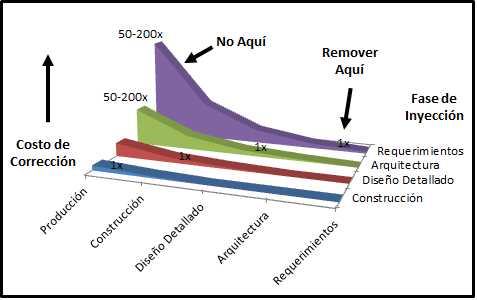
\includegraphics[scale=0.9]{images/DefectCost.png}
	\caption{Costo de la Remoci'on de Defectos por Fase}
	\label{fig:DefectCost}
\end{figure}

El costo de remover un defecto de software crece exponencialmente cada fase que este se mantiene dentro del ciclo de desarrollo sin ser detectado\cite{Boehm1981}. En un proyecto t'ipico de software, el 80\% del costo total es utilizado en la correcci'on de defectos\cite{Lazic2009}.

Es por esto que el BM sugiere una cultura de revisi'on y prevenci'on, la cual tiene como objetivo evitar la introducci'on de defectos, removerlos tan r'apido como sea posible si es que estos son inyectados y as'i evitar el aumento exponencial de costo y esfuerzo. El BM sugiere que la calidad en el desarrollo de software es mucho m'as que simplemente introducir una fase de pruebas. Las iniciativas de calidad deben existir durante todo el proceso de desarrollo para alcanzar la meta de un software con cero defectos.

\section{Costo de la Calidad de Software}
\noindent
El Costo de la Calidad (por sus siglas en Ingl�s CoQ) representa los costos en los que incide una organizaci�n al tener que repetir un proceso para realizar el trabajo correctamente\cite{Lazic2009}. El CoQ es un t�rmino que nos permite evaluar la econom�a involucrada para producir software de alta calidad\cite{Lazic2009}.
El CoQ se divide en dos tipos principales: El costo de la conformidad y el costo de la no conformidad\cite{Black2002}.

\begin{math}CoQ = Costo_{Conformidad} + Costo_{No-conformidad}\end{math}

A su vez, el costo de la conformidad se divide en costos de prevenci�n y costos de evaluaci�n, mientras que el costo de la conformidad se divide en fallas internas y externas\cite{Houston1998}. Esto se muestra en la figura\ref{fig:CoQ}:

\begin{math}CoQ = Prevencion_{Costo} + Evaluacion_{Costo} + FallasInternas_{Costo} + FallasExternas_{Costo}\end{math}

\begin{figure}[h]
	\centering
		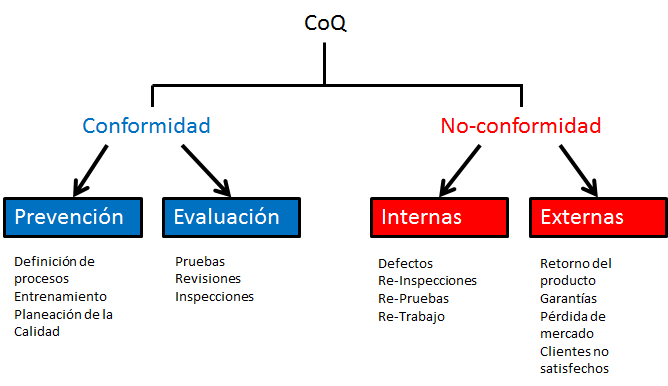
\includegraphics[scale=0.9]{images/CoSQ.png}
	\caption{Costo de la Calidad de Software}
	\label{fig:CoQ}
\end{figure}

Los significados los diferentes tipos de costos son los siguientes\cite{Juran1998}:

\begin{itemize}
	\item \emph{Costos de prevenci�n}. Son los costos asociados con la planeaci�n de la calidad; el dise�o, la implementaci�n y la administraci�n de la calidad del sistema; la auditor�a del sistema; encuestas a los proveedores y las mejoras de proceso.
	\item \emph{Costos de evaluaci�n}. Son los costos asociados con la medici�n, evaluaci�n y revisi�n de los productos para asegurar su conformidad con los est�ndares de calidad y requerimientos de desempe�o.
	\item \emph{Costos de falla}. Son las p�rdidas asociadas con la creaci�n de un producto que no cumpla con los criterios de conformidad. Se dividen en internos y externos.
	\item \emph{Costos de falla internos}. Son los costos asociados con las fallas y defectos del proceso, equipo, producto y materiales que no cumplen con los est�ndares de calidad o los requerimientos.
	\item \emph{Costos de falla externos}. Son generados por productos, servicios y procesos defectuosos cuando el usuario los utiliza. Incluyen garant�as, quejas, devoluciones y remplazos.
\end{itemize}

La figura \ref{fig:CoQ-Graph} es una representaci�n gr�fica del CoQ propuesta por varios investigadores\cite{Knox1993,Houston1998,Black2002}.

\begin{figure}[h]
	\centering
		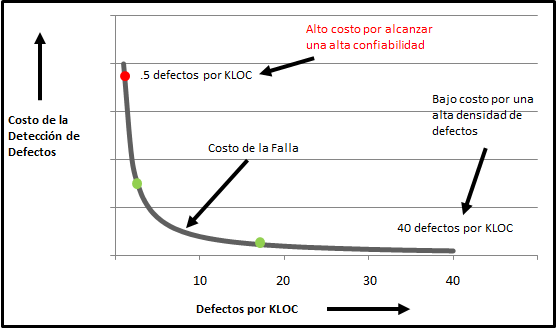
\includegraphics[scale=0.9]{images/CoSQ-Graph.png}
	\caption{El costo de la alta confiabilidad}
	\label{fig:CoQ-Graph}
\end{figure}

La figura anterior nos muestra que para alcanzar una alta confiabilidad y cero defectos (cerca del punto rojo) el costo es muy alto, pero alcanzar un nivel razonable de calidad (entre los dos puntos verdes) no requiere un costo muy alto.

\subsection{De las Pruebas a la Prevenci'on}
\noindent
Anteriores esquemas de calidad de software suger'ian que una fuerte etapa de pruebas era la mejor acci'on posible para asegurar la calidad en el software, sin embargo, una encuesta dirigida por \cite{Lazic2009} a distintas organizaciones dedicadas al desarrollo de software encontr'o que la mayor'ia de estas organizaciones estaban de acuerdo que una cultura que favoreciera las pruebas antes que la prevenci'on de los defectos provocaba un programa poco productivo de calidad.

Los costos para dar calidad y los costos causados por falta de la calidad tienen una relaci'on inversa: mientras que la inversi'on en alcanzar calidad aumenta, los costos provocados por la falta de calidad disminuyen\cite{Lazic2009}. Este modelo te'orico se muestra en la figura \ref{fig:ModelOfSQ}\cite{Lazic2009}. La figura muestra que mientras los costos de prevenci'on y evaluaci'on aumentan, los costos de las fallas disminuyen hasta que se alcanza un punto 'optimo, despu'es del punto 'optimo aumentar la inversi'on en prevenci'on y evaluaci'on no tienen tan buenos resultados \cite{Lazic2009}.

\begin{figure}[h]
	\centering
		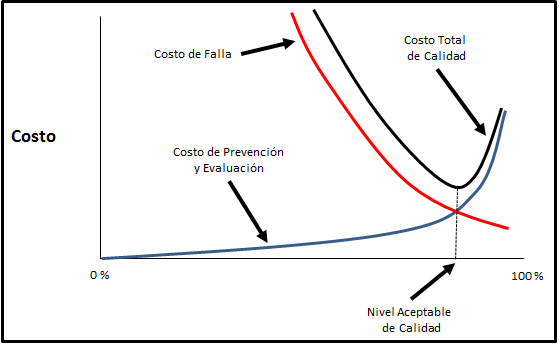
\includegraphics[scale=0.9]{images/ModelOfSQ.png}
	\caption{Modelo de la Calidad de Software}
	\label{fig:ModelOfSQ}
\end{figure}

Cuando se comienza a invertir en evaluaci'on provoca que las fallas internas aumenten ya que se detectan m'as defectos en etapas tempranas, pero remover defectos en etapas tempranas es mucho m'as barato que hacerlo en pruebas o mantenimiento\cite{Lazic2009}. En general las actividades de evaluaci'on disminuyen las fallas externas y el total de fallas disminuye. Una inversi'on peque'na en prevenci'on y evaluaci'on produce grandes disminuciones de costo total de calidad\cite{Lazic2009}.

Fomentar una cultura donde la prevenci'on de los errores sea m'as importante que el proceso de pruebas es uno de los objetivos de este trabajo de Tesis.

\subsection{An'alisis del Costo de la Calidad}
\noindent
El an'alisis del costo de la calidad es el concepto de estudiar los costos relacionados con la calidad como medios de comunicaci'on entre el departamento de calidad y la gerencia de las organizaciones\cite{Lazic2009}. El objetivo de hacer un an'alisis del costo de la calidad no es reducir el costo, si no asegurarnos de que se invierta en el tipo correcto de costo y se maximice el beneficio obtenido de esa inversi'on. La mejor estrategia para esto es cambiar las actividades relacionadas con las fallas por actividades de prevenci'on y evaluaci'on. 

Un an'alisis costo beneficio se realiza para determinar que tan bien, o que tan mal, una acci'on resultar'a. Un an'alisis de costo beneficio encuentra, cuantifica y agrega los factores positivos. Estos son los beneficios, entonces cuantifica y substrae todos los negativos, en otras palabras los costos. La diferencia entre estos indica si la acci'on es recomendable o no\cite{Lazic2009}.

Una consideraci'on clave en el an'alisis del costo de la calidad es la visibilidad. La visibilidad obtenida gracias al an'alisis del costo de la calidad permite el equipo de aseguramiento de la calidad enfocar su atenci'on en aquellas actividades que descubren y corrigen la causa ra'iz de los defectos. La causa ra'iz puede ser utilizada para determinar como el proceso de desarrollo puede ser mejorado para prevenir nuevos defectos\cite{Lazic2009}.

Knox propone un modelo te'orico en el cual demuestra la inversi'on en las distintas actividades del CoQ seg'un el nivel de CMMI\cite{Knox1993}. Este se muestra en la figura \ref{fig:CoQ-CMM} donde podemos observar como se reduce el CoQ total al ir aumentando las actividades de evaluaci'on y prevenci'on seg'un el nivel de CMMI.

\begin{figure}[h]
	\centering
		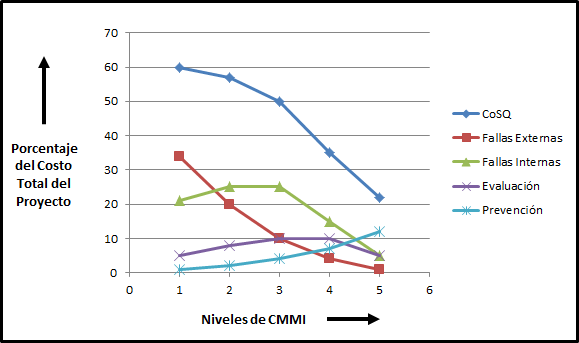
\includegraphics[scale=0.9]{images/CoSQ-CMM.png}
	\caption{CoQ por nivel de CMM}
	\label{fig:CoQ-CMM}
\end{figure}

Para hacer una mejora real en la calidad de software debemos enfocarnos en dos mejoras de proceso\cite{Lazic2009}: Prevenci'on de defectos y remoci'on de defectos.

La prevenci'on de defectos se refiere a las tecnolog'ias y metodolog'ias que reducen el n'umero de defectos que deben de ser eliminados. Ejemplos de estos m'etodos pueden ser m'etodos formales de dise'no, generaci'on autom'atica de c'odigo a partir de especificaciones formales, la capacitaci'on y la creaci'on de una conciencia sobre los defectos inyectados.

La remoci'on de defectos se refiere a los m'etodos que pueden aumentar los niveles de eficiencia en la remoci'on de defectos al introducir diferentes tipos de revisiones.


\subsection{An'alisis del Retorno de Inversi'on}
\noindent
Hay dos beneficios principales de tener una alta calidad en el software: Tiempo y dinero. El retorno de inversi'on (por sus siglas en Ingl'es ROI) analiza los ahorros en costo y en calendario que se tienen al implementar ciertas actividades de calidad\cite{Lazic2009}. El ROI se expresa en t'erminos de esfuerzo ya que es el mayor costo de un proyecto de software.

Una forma de calcular el ROI de un proyecto es la siguiente\cite{Lazic2009}:

\begin{math}ROI = \frac{OriginalTotalCoQ - NewTotalCoQ}{OriginalTotalCoQ}\end{math}

Este modelo nos muestra el porcentaje de ahorro del costo de calidad total del proyecto. Para ilustrarlo se muestra un ejemplo en la tabla \ref{ROItable}\cite{Lazic2009}. En esta tabla se muestran dos casos hipot'eticos, en ambos se trata de un proyecto con mil defectos. El primero muestra el CoQ de una empresa que no invierte en prevenci'on y evaluaci'on, mientras que en el segundo caso se muestra el escenario donde se realiza la inversi'on. De esta manera se calcula el ROI, realizando la comparaci'on de los costos que se hubieran tenido sin una estrategia de calidad, contra el CoQ real.

\begin{table}[htbp]
	\centering
		\begin{tabular}{| c | c | c |}
		  \hline
		  \multicolumn{3}{|c|}{\textbf{An'alisis del ROI}} \\
		  \hline
		  \textbf{Recursos} & \textbf{Caso1} & \textbf{Caso2} \\
		  Personal & \$0 & \$60,000 \\
		  Infraestructura & \$0 & \$10,000 \\
		  Herramientas & \$0 & \$12,500 \\
		  Total de Inversi'on & \$0 & \$82,500 \\
		  \hline
		  \multicolumn{3}{|c|}{\textbf{Desarrollo (Requerimientos, Dise�o y Codificaci'on)}} \\
		  \hline
		  Defectos Encontrados & 250 & 350 \\
		  Costo de Correcci'on de Defectos & \$2,500 & \$3,500 \\
		  \hline
		  \multicolumn{3}{|c|}{\textbf{Pruebas}} \\
		  \hline
		  Defectos Encontrados & 0 & 600 \\
		  Costo de Correcci'on de Defectos & 0 & \$60,000 \\
		  \hline
		  \multicolumn{3}{|c|}{\textbf{Producci'on}} \\
		  \hline
		  Defectos Encontrados & 750 & 50 \\
		  Costo de Correcci'on de Defectos & \$750,000 & \$50,000 \\
		  \hline
		  \hline
		  \multicolumn{3}{|c|}{\textbf{CoQ}} \\
		  \hline
		  Conformidad & 0 & \$82,500 \\
		  No-conformidad & \$752,500 & \$113,500 \\
		  \textbf{Total} & \$752,500 & \$196,000 \\
		  \textbf{ROI} & NA & 74\% \\
		  \hline
		\end{tabular}
	\caption{An'alisis del ROI}
	\label{ROItable}
\end{table}

\begin{math}ROI = \frac{752500 - 196000}{752500}=0.74=74\%\end{math}

Este resultado nos quiere decir que se ahorr'o el 74\% del total de CoQ. Estos an'alisis son realizados com'unmente antes al finalizar las pruebas de sistema y antes de ingresar a producci'on. Por lo cual la situaci'on del ROI puede empeorar conforme el sistema se encuentra en producci'on y los usuarios comienzan a encontrar los defectos mientras lo usan.


\clearpage